\documentclass[a4paper,12pt,oneside,onecolumn]{article}
\usepackage[utf8]{inputenc}
\usepackage[italian]{babel}
\usepackage{hyperref}
\usepackage[round,numbers]{natbib}
%\usepackage{listings}
%\usepackage{graphicx}
%\usepackage{amsmath}
\usepackage[T1]{fontenc}
\usepackage{lmodern}
%\usepackage[scaled=0.9]{beramono}
%\usepackage{microtype}
\usepackage{color}
\usepackage{xcolor}
%\usepackage{float}
\usepackage{lipsum}
\usepackage[noadvisor,swapnames]{frontespizio}
\usepackage{minted}
\definecolor{light-gray}{gray}{0.95}

\renewcommand*\rmdefault{iwona}

\usemintedstyle{default}

\newminted{prolog}
{ 
  frame=lines,
  framesep=2mm,
  baselinestretch=1,
  bgcolor=light-gray,
  fontsize=\small,
  linenos
}

\newminted{java}
{ 
  frame=lines,
  framesep=2mm,
  baselinestretch=1,
  bgcolor=light-gray,
  fontsize=\footnotesize,
  linenos
}

\begin{document}

    \begin{frontespizio}
        \Universita {Bari ``Aldo Moro"}
        \Logo [2cm]{./img/logo}
        \Dipartimento{Informatica}
        \Corso [Laurea]{Informatica Magistrale}
        \Titoletto {Documentazione di progetto di Intelligenza Artificiale}
        \Titolo{Text Extraction in ambito giuridico}
        \NCandidati{Studenti}
        \Candidato{Luciano Quercia}
        \Candidato{Simone Rutigliano}
        \Annoaccademico {2013-2014}
        \Margini{4cm}{4.5cm}{4cm}{4cm}
    \end{frontespizio}

\section{Introduzione}

\subsection{Sistemi esperti per la configurazione}

\subsection{Scopo del progetto}
\section{Studio del dominio}
\subsection{Descrizione del dominio}
\subsection{Studio del dominio e fonti utilizzate}
\subsection{Individuazione delle componenti di un sistema}
\subsection{Individuazione dei bisogni dell’utente}
\section{Progettazione}

\subsection{Obiettivo}
Come primo obiettivo, il sistema deve essere in grado di estrarre, da documenti testuali, alcune informazioni principali, quali:
\begin{itemize}
\item numero della pratica; %TODO
\item soggetto della richiesta di iscrizione;
\item quantità di denaro richiesta e tipologia.
\end{itemize}

Come feature aggiuntive, il sistema si può occupare dell'estrazione, su richiesta, di altre informazioni utili come:
\begin{itemize}
\item indirizzi email;
\item numeri di telefono;
\item nomi di comuni;
\item altre persone nominate nel testo;
\item etc.
\end{itemize}


\subsection{Input e Assunzioni}
Non avendo a disposizione dei documenti di input reali sui quali il sistema deve essere in grado di lavorare e, quindi, non conoscendone il formato o la composizione, abbiamo dovuto fare delle assunzioni e realizzare degli esempi di input ad hoc.
Per essere pronti a successivi adattamenti, abbiamo fatto le scelte meno vantaggiose, ipotizzando di non avere a disposizione alcuna strutturazione nel documento o metadati su di esso.
I nostri esempi di input sono delle semplicissime stringhe prive di \verb+newline+, tabulazioni, ordinamento nello spazio, tag di qualsiasi tipo.
Nel caso in cui in futuro dovessimo essere in possesso di alcune di queste informazioni, potremmo utilizzarle per migliorare le nostre regole.


\subsection{Strategia risolutiva}
Il problema che affronteremo rientra nell'ambito dell'\emph{Information Extraction}, un task di Intelligenza Artificiale che mira all'estrazione automatica di informazioni strutturate da documenti non-strutturati o semi-strutturati.

Nella maggior parte dei casi, questa attività riguarda l'elaborazione di testi scritti in linguaggio naturale (NLP).

Abbiamo deciso di servirci di alcune delle tecniche di analisi lessicale e sintattica già note e utilizzate in questo campo.

\subsubsection{Lexical Analysis}
Il testo in input (come già detto testo semplice in una stringa) deve subire una pre-elaborazione lessicale, con l'obiettivo di ottenere una lista di token 

\subsection{Oggetti del dominio}
Per poter estrarre le informazioni a più alto livello quali, ad esempio, \emph{soggetto} e \emph{quantità di denaro richiesta}, dobbiamo utilizzare numerosi oggetti, specifici del dominio giuridico e non.

\subsubsection{Persone}
Per l'individuazione delle persone fisiche presenti nel testo (oltre al soggetto della richiesta, anche il giudice, l'avvocato o altre persone nominate nel testo) è utile riuscire a distinguere un \fbox{nome} e un \fbox{cognome}, eventuali \fbox{titoli} quale 


\subsection{Individuazione delle funzioni}

\subsection{Individuazione delle relazioni}

\subsection{Dalla concettualizzazione alle regole}


\section{Implementazione}

\subsection{Architettura del sistema}
Per preservare l'indipendenza delle componenti del sistema, abbiamo realizzato dei moduli Prolog che espongano pubblicamente solo i predicati necessari.

Il file \verb+main.pl+ costituisce l'entry-point del programma, l'unico file necessario da importare nell'interprete per l'esecuzione.

Come anticipato nella sezione~\ref{sec:Progettazione}, il sistema è composto principalmente da un \emph{lexer} e da un \emph{tagger}.

Lo schema delle dipendenze è mostrato in figura~\ref{fig:moduli}.

\begin{figure}[h!tbp]
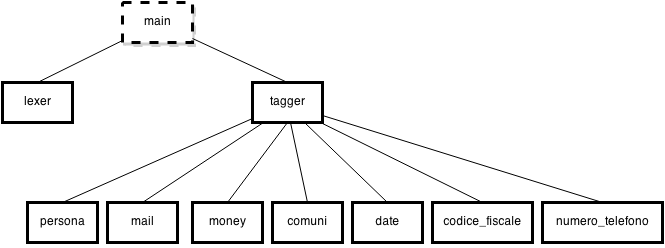
\includegraphics[width=\textwidth]{img/struttura_moduli.png}
\label{fig:moduli}
\end{figure}

\subsection{Lexer}
Il compito del \emph{lexer} sarà quello di normalizzare la stringa contenente il documento da analizzare in una lista di token su cui poi il tagger dovrà fare le sue analisi. Per fare ciò, bisognerà nell'ordine: 
\begin{itemize}
    \item ripulire la stringa di stopchars;
    \item separare i caratteri speciali (punto, virgola, euro e chiocciola) da eventuali caratteri a cui sono associati;
    \item eliminare eventuali spazi bianchi superflui causati da eliminazioni di caratteri fatte in precedenza;
    \item rendere case insensitive la stringa ripulita.
\end{itemize}
Di seguito il predicato lexer:

\begin{prologcode}
lexer(String,ListToken) :-
    filter_stopchars(String, A),
    clean_chiocciola(A,B),
    clean_punto(B,C),
    clean_virgola(C,D),
    clean_euro(D,E),
    strip_spaces(E, F),
    atom_codes(G, F),
    atomic_list_concat(H,' ', G),
    maplist(downcase_atom, H, ListToken).
\end{prologcode}

\subsection{Tagger}
Il compito del \emph{tagger} invece, sarà quello di individuare in maniera deterministica le componenti salienti del testo cosi come detto in precedenza nel paragrafo \ref{tagger}.

Di seguito verrà riportato il predicato tagger:

\begin{prologcode}
tagger(ListToken,ListTagged) :-
    tag_persona(ListToken,A),
    tag_indirizzo(A,A1),
    tag_mail(A1,B),
    tag_money(B,C),
    tag_date(C,D),
    tag_comune(D,E),
    tag_cf(E,F),
    tag_numero_telefono(F,G),
    filter_stopwords(G,ListTagged).
\end{prologcode}

\subsection{Persone}
Al fine di individuare tutte le persone fisiche, con i rispettivi ruoli, all'interno del documento, è stato necessario utilizzare la tecnica del divide et impera. In questo modo, in prima battuta, sono stati individuati contemporaneamente tutte le possibili persone e tutti i probabili ruoli che una persona può avere, quali ad esempio (colui che creditore verso l'entità fallita, commissario, giudice, curatore, avvocato,etc.).

Per verificare se una sequenza di token può considerarsi essere una persona, sono stati presi in esame tutte le possibili combinazioni di nomi e cognomi che una persona italiana può avere secondo lo stato italiano; si potranno avere infatti, fino ad un massimo di due cognomi concatenati a tre nomi o la sua commutazione. Inoltre, affinché fosse verificato che un token sia un nome o un cognome, è stata utilizzata una base di conoscenza prolog contenente un buon quantitativo di nomi e cognomi italiani.

Successivamente si andranno a unificare i ruoli trovati con le persone più vicine a quei ruoli, creando cosi l'entità finale composta da persona e ruolo.
Inoltre, il predicato terrà anche in considerazione il fatto che in un documento ci sia la probabilità che la persona, oltre al ruolo abbia anche uno o più aggettivi a lui associato (e.g. Ill.mo Giudice Mario Bianchi); in questo caso, gli aggettivi non verranno presi in considerazione nel tag finale.

Inoltre, è stato realizzato il predicato \emph{tag\_indirizzi} che avrà il compito di evitare che vengano taggate persone presenti in indirizzi postali.

Di seguito il predicato \emph{tag\_persona} che permette la realizzazione del tag descritto:

\begin{prologcode}
tag_persona(List,ListTagged) :-
    tag_aggettivo(List,A),
    tag_ruolo(A,B),
    strip_aggettivi(B,C),
    tag_nome(C,D),
    tag_titolo(D,ListTagged).
\end{prologcode}

\subsection{Richiesta di denaro}
La seconda entità principale che il tagger andrà a ricercare all'interno del documento sarà il quantitativo di denaro che il creditore andrà a richiedere al debitore. Per fare ciò, si seguirà la stessa linea di pensiero usata per il tag precedente, nella fattispecie, in una prima fase si andranno ad individuare sia tutte le possibili cifre di denaro presenti nel documento, sia tutte le tipologie di richieste che si potranno fare (chirografario, privilegiato e totale); nella seconda fase, invece, si andranno ad unificare le due entità più vicine di questi due tipi.

Per quanto riguarda l'individuazione delle cifre di denaro, sono state prese in considerazione tutte le possibili combinazioni di valore e valuta (e.g. 20\texteuro, \textdollar 20, 20 eur, etc.).

Invece, per l'individuazione delle tipologie di richieste, si è preferito uniformare le tipologie ad una singola parola per tipologia (e.g. chirografario, chirografaria, chirografo, chirografa, chiro e chir verranno tutte ricondotte al termine \emph{chirografario}).

Di seguito il predicato \emph{tag\_money} in grado di eseguire le operazioni descritte nel paragrafo.

\begin{prologcode}
tag_money(A,F) :- 
    tag_currency(A,B),
    tag_chirografario(B,C),
    tag_privilegiato(C,D),
    tag_totale(D,E),
    tag_richiesta(E,F).
\end{prologcode}

\subsection{Informazioni aggiuntive}

%TODO
%tag\_mail
%tag\_date
%tag\_comune
%tag\_cf
%tag\_numero\_telefono
%filter\_stopwords

%TODO JPL DEPRECATED LIST

\subsection{Le regole}
\subsection{L'inferenza}
\section{Componenti aggiuntive}
\subsection{Gestione dell'incertezza}
\subsection{Come e perché}
\subsection{Interazione con l'utente}
\subsection{Alcune funzioni utili}
\section{Descrizione del sistema}

Il sistema presenta un'interfaccia grafica in grado di permettere l'interazione con il core del sistema scritto in Prolog, dando cosi la possibilità a qualunque tipo di stakeholders del sistema di utilizzarlo senza la necessità di dover interagire con il terminale, rendendo cosi le informazioni più leggibili e usabili; Oltre a questo, la creazione dell'interfaccia permette anche di evitare possibili errori dattilografici che si potrebbero avere in caso di interazione con il terminale.

Gli elementi principali dell’interfaccia, con i relativi pulsanti, la cui funzione e uso verranno descritti in dettaglio nel prossimo paragrafo, sono i seguenti (nella figura 1, i numeri delle aree corrispondono alle rispettive funzioni assegnate enumerate
nell’elenco seguente):
\begin{itemize}
	\item Sezione di inserimento del documento da cui si devono estrarre le informazioni
	\item Sezione di scelta delle informazioni da estrarre
	\item Sezione di visualizzazione dei risultati ottenuti
\end{itemize}
\subsection{Sezioni ed operazioni disponibili}
    \subsubsection{Inserimento}
    \label{Inserimento}
    In questa sezione viene data la possibilità di inserire il documento testuale da cui si vogliono estrarre le informazioni; con questa operazione non si fa altro che asserire un documento da dover poi essere processato dal core prolog del sistema.
    \subsubsection{Scelta dei tag}
    \label{ChoiceTag}
    In questa sezione si da la possibilità all'utente di filtrare i tag da voler estrarre dal documento attraverso la selezione/deselezione della checkbox corrispondente al tag; con questa operazione si vanno a selezionare quali saranno i tag che il core prolog deve etichettare nel documento.
    \subsubsection{Visualizzazione}
    \label{Visualization}
    In questa schermata invece verranno mostrate le informazioni che l'utente ha deciso di estrarre dal documento; inoltre le diverse tipologie di tag saranno evidenziate diversamente l'uno dall'altro attraverso l'ausilio di una colorazione dei tag. 

    \subsubsection{Reset delle condizioni iniziali}
    Tramite il pulsante \emph{Reset} si ripristinano le condizioni iniziali del sistema.In particolare, viene ripristinato lo stato iniziale:
    \begin{itemize}
    	\item \emph{Interfaccia} : cancellando le textbox contenenti il documento inserito \ref{Inserimento} e i tag etichettati dal testo \ref{Visualization}, sia le scelte dei tag da effettuare \ref{ChoiceTag}.
    	\item \emph{Core Prolog} : ritrattando il documento appena inserito nella sezione \ref{Inserimento}.
    \end{itemize}
    
\subsection{Interazione con l’utente}
L’interazione avviene principalmente tramite l'interfaccia grafica descritta nella sezione precedente ma viene data anche la possibilità di interagire con il sistema anche senza l'ausilio di tale interfaccia, utilizzando direttamente l'interprete Prolog da terminale, previa consultazione del modulo principale del sistema denominato \emph{main.pl}; le funzionalità del sistema sono indipendenti dal metodo con cui si vuole interagire con il  sistema. Qualora si volesse tener traccia anche di come avviene la comunicazione tra java e prolog, è possibile visionare tale interazione all'interno della finestra di terminale da cui si è lanciato il sistema.

\subsubsection{JPL Library}
La libreria utilizzata per permettere la bidirezionalità della comunicazione tra Java e Prolog, è stata la \emph{JPL 3.1.4 alpha}\footnote{Scaricabile da \url{http://mvnrepository.com/artifact/jpl/jpl/3.1.4-alpha}} (\textbf{J}ava-calls-\textbf{P}rolog \textbf{L}ibrary)


The JPL 3.0.1 Java-calls-Prolog API provides a set of classes that hide almost all of the messy detail in the Low-Level Interface.  It is less flexible than the Low-Level Interface, but it also has less of a learning curve, and in many ways is more natural and Prolog-like than the Low-Level Interface.

The Java package jpl contains all of the classes in this interface.  None of the classes correspond with any of the data types in the Prolog Foreign Language Interface (FLI). 


The Class Hierarchy

The API consists of the following class hierarchy:
\begin{Verbatim}
Term
|
+--- Variable
|
+--- Compound
|      |
|      +--- Atom
|
+--- Integer
|
+--- Float

Query

JPLException
|
+-- PrologException
\end{Verbatim}
\begin{Verbatim}
Term is an abstract class: only its subclasses can be instantiated.

Each instance of Query contains a Term (denoting the goal which is to be proven), and much more besides.

Each instance of Compound has a (java.lang.String) name and an array of (Term) arguments (it must have at least one).

Atom is a specialisation of Compound with zero arguments. 

  JPL.setNativeLibraryDir(yapJPLPath);
  
  prolog.consult(new Atom("prolog/main.pl"));
  prolog.retractAll("domanda", 1);
  Term toAssert = new Compound("domanda", new Term[]{Util.textToTerm("\"" + textPane.getText() + "\"")});
  prolog.asserta(toAssert);
  java.util.Hashtable<String, Term>[] hashtables = prolog.allSolutions(new Compound("nextTag", new Term[]{new Variable("Tag")}));
  
  \end{Verbatim}
  \begin{javacode}
package it.uniba.di.ia.ius;

import jpl.*;

public class Prolog {
  
  public boolean consult(Atom atom) {
    Term t = new Compound("consult", new Term[]{atom});
    Query query = new Query(t);
    System.out.print("[Prolog] consult: " + t + " ");
    System.out.println(query.hasSolution() ? "succeeded" : "failed");
    return query.hasSolution();
  }
  
  public void asserta(Term term) {
    Term t = new Compound("asserta", new Term[]{term});
    Query query = new Query(t);
    System.err.print("[Prolog] asserta( " + term + " ) ");
    System.err.println(query.hasSolution() ? "succeeded" : "failed");
  }
  
  public void assertz(Term term) {
    Term t = new Compound("assertz", new Term[]{term});
    Query query = new Query(t);
    System.err.print("[Prolog] assertz( " + term + " ) ");
    System.err.println(query.hasSolution() ? "succeeded" : "failed");
  }
\end{javacode}

\begin{javacode*}{firstnumber=29}  
  public void retract(Term term) {
    Term t = new Compound("retract", new Term[]{term});
    Query query = new Query(t);
    System.err.print("[Prolog] retract( " + term + " ) ");
    System.err.println(query.hasSolution() ? "succeeded" : "failed");
  }
  
  public void retractAll(String predicate, int arity) {  
    Term[] args = new Term[arity];
    for (int i = 0; i < args.length; i++)
    args[i] = new Variable("_");
    
    Term[] termToRetract = new Term[]{ new Compound(predicate, args) };
    
    Term t = new Compound("retractall", termToRetract);
    Query query = new Query(t);
    System.err.print("[Prolog] retract( " + predicate + " ) ");
    System.err.println(query.hasSolution() ? "succeeded" : "failed");
  }
  
  public boolean statisfied(Term t) {
    Query query = new Query(t);
    System.err.print("[Prolog] query: " + t + " ");
    System.err.println(query.hasSolution() ? "succeeded" : "failed");
    return query.hasSolution();
  }
  
  public java.util.Hashtable oneSolution(Term t) {
    Query query = new Query(t);
    System.err.print("[Prolog] query: " + t + " ");
    System.err.println(query.hasSolution() ? "succeeded" : "failed");
    return query.oneSolution();
  }
  
  public java.util.Hashtable[] nSolutions(Term t, long size) {
    Query query = new Query(t);
    System.err.print("[Prolog] query: " + t + " ");
    System.err.println(query.hasSolution() ? "succeeded" : "failed");
    return query.nSolutions(size);
  }
  
  public java.util.Hashtable[] allSolutions(Term t) {
    Query query = new Query(t);
    System.err.print("[Prolog] query: " + t + " ");
    System.err.println(query.hasSolution() ? "succeeded" : "failed");
    return query.allSolutions();
  }
}
    \end{javacode*}
    

\subsection{Esempio di interazione}

\subsection{Utilizzo della funzione spiega domanda}

\subsection{Presentazione dei risultati}

\subsection{Utilizzo della funzione spiega ragionamento}


\bibliographystyle{abbrvnat}
\bibliography{mybib}

\end{document}